\section{実験目的}
本プロジェクトでは、雑多な環境下で人追従でき、ロボットの最大直進速度で追従できる人追従システムの
開発を目的としている。これに伴った実験の目的は、雑多な環境下での人追従の精度とロボットの
最大直進速度での人追従性能の2つの検証をすることである。以上のことから、追従実験と最大
追従速度実験により、開発した人追従システムの性能を検証する。

\section{実験方法}
実験では、雑多な環境下での追従性能を検証する追従実験と、
ロボットの最大直進速度での追従を検証する最大追従速度実験をする。
実験中は、人は追従対象の1人のみとする。\\ \indent
要求仕様(2)を検証するため、追従実験では直線経路、曲線経路、直角経路をそれぞれ10回実験し、
成功率を算出する。追従の成功率が各経路において90\%以上であった場合に要求仕様(2)を満たしたものとする。
また、要求仕様(3)を検証するため、10[m]以上の直線経路にて最大追従速度実験をする。
0.1[m/s]から、0.1ずつ速度を上昇させ、追従できなくなる速度の直前を最大追従速度とする。
Turtlebot3 Big Wheelの最大直進速度が0.5[m/s]であるため、開発した人追従システムの
最大追従速度が0.5[m/s]であった場合に要求仕様(3)は満たされる。
以上の実験は、2D-LiDARのデータを用いた実験であるため、要求仕様(2)、(3)が満たされたら、
要求仕様(1)も満たされたものとする。

\subsection{実験機材}
本プロジェクトでは、2023年に開催されたRoboCup2023で開発したHappy Eduを使用する。
Happy Eduの全体像をFig. \ref{Happy Edu}に示す。Happy Eduに搭載するノートPCは、ASUSの
ROG Strix G16を用いている。ロボット台車には、ROBOTIS社の二輪差動駆動台車である
TurtleBot3 Big Wheelを用いてる。2D-LiDARには、北洋電機株式会社のUTM30-LXを用いている。
ノートPC、ロボット台車、2D-LiDARの仕様は、それぞれ
Table \ref{ASUS ROG Strix G16 specification}、
Table \ref{TurtleBot3 Big Wheel specification}、
Table \ref{UTM30-LX specification}に示す。

\begin{figure*}[h]
  \begin{center}
  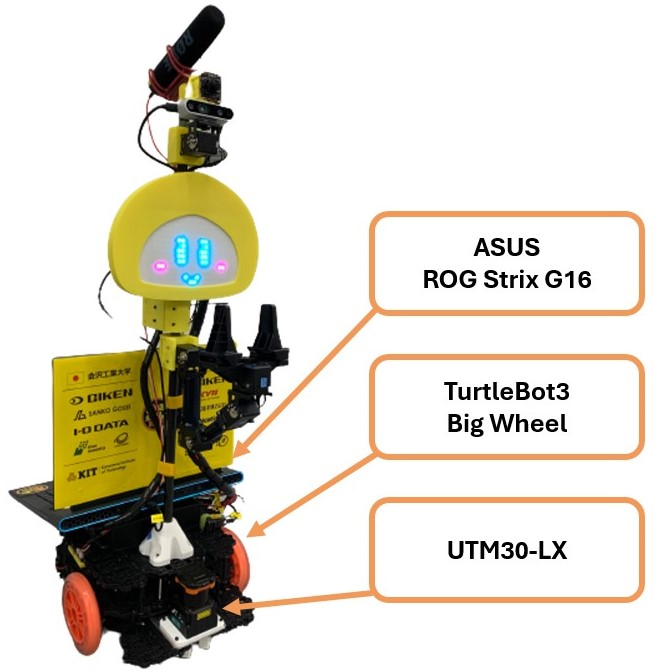
\includegraphics[width=60mm,clip]{figure/Happy_Edu.jpg}
  \caption{Happy Edu}
  \label{Happy Edu}
  \end{center}
\end{figure*}

\begin{table}[h]
  \begin{center}
    \caption{{ASUS ROG Strix G16 specification}\label{ASUS ROG Strix G16 specification}}
    \scalebox{1.2}[1.0]{
      \begin{tabular}{c|c} \hline
        Size & 264.0 x 354.0 x 22.6[mm]  \\ \hline
        Weight & 2500[g] \\ \hline
        Model & G614JI-I7R4070 \\ \hline
        Form factor & laptop \\ \hline
        Resolution & 1920 x 1200 [pixel] \\ \hline
        CPU & Intel Corei7 13650HX \\ \hline
        RAM & 32[GB] \\ \hline
        GPU & NVIDIA GeForce RTX 4070 \\ \hline
        VRAM & 8[GB] \\ \hline
      \end{tabular}
    }
  \end{center}
\end{table}

\begin{table}[h]
  \begin{center}
    \caption{{TurtleBot3 Big Wheel specification}\label{TurtleBot3 Big Wheel specification}}
    \scalebox{1.0}[0.9]{
      \begin{tabular}{c|c} \hline
        Maximum straight speed & 0.5[m/s] \\ \hline
        Maximum rotation speed & 3.14[rad/s] \\ \hline
        Maximum payload & 30[kg] \\ \hline
        Size & 281 x 306 x 170.3 [mm] \\ \hline
        Actuator & XM430-W210 \\ \hline
        Supply input terminal & 3.3[V] / 800[mA], 5[V] / 4[A], 12[V] / 1[A] \\ \hline
        Battery & Lithium polymer 11.1[V] 1800[mAh] / 19.98[Wh] 5[C] \\ \hline
      \end{tabular}
    }
  \end{center}
\end{table}

\begin{table}[h]
  \begin{center}
    \caption{{UTM30-LX specification}\label{UTM30-LX specification}}
    \scalebox{1.0}[0.9]{
      \begin{tabular}{c|c} \hline
        Power source & 12[V]DC \\ \hline
        Current consumption & 700[mA] \\ \hline
        Scanning range & 0.1 to 30[m] \\ \hline
        Scanning angle & 270 [deg] \\ \hline
        Angular Resolution & Step angle: approx.0.25[deg](360[deg]/1,440[steps]) \\ \hline
        Scanning time & 25[msec]/scan \\ \hline
        Weight & 210[g] \\ \hline
      \end{tabular}
    }
  \end{center}
\end{table}

\subsection{追従実験}
要求仕様(2)を検証するため、
Fig. \ref{Image of tracking experiment environment (FMT Laboratory Room 206)}と
Fig. \ref{Image of tracking experiment environment (FMT Laboratory Room 326)}
のような雑多な環境を用意し、追従の成否を実験する。
雑多な環境の用意では、人の脚部と類似している椅子やポールなどの円柱状の物体を多く
設置している。\\ \indent
直線経路、曲線経路、直角経路のイメージをそれぞれ
Fig. \ref{Straight road}、Fig. \ref{Curved road}、Fig. \ref{Right angle road}に示す。
直線経路、曲線経路、直角経路においてそれぞれ10回ずつ試行し、各径路での追従成功率を算出する。
追従が成功した回数を$x_{success}$とした時の追従成功率$success \; rate$は以下のようになる。

\begin{equation}
\label{Success rate}
  success \; rate = x_{success} / 10
\end{equation}

(\ref{Success rate})式を用いて各径路での成功率を算出し、それぞれの成功率が90[\%]以上
であれば要求仕様(2)を満たしたこととする。

\begin{figure*}[h]
  \begin{center}
  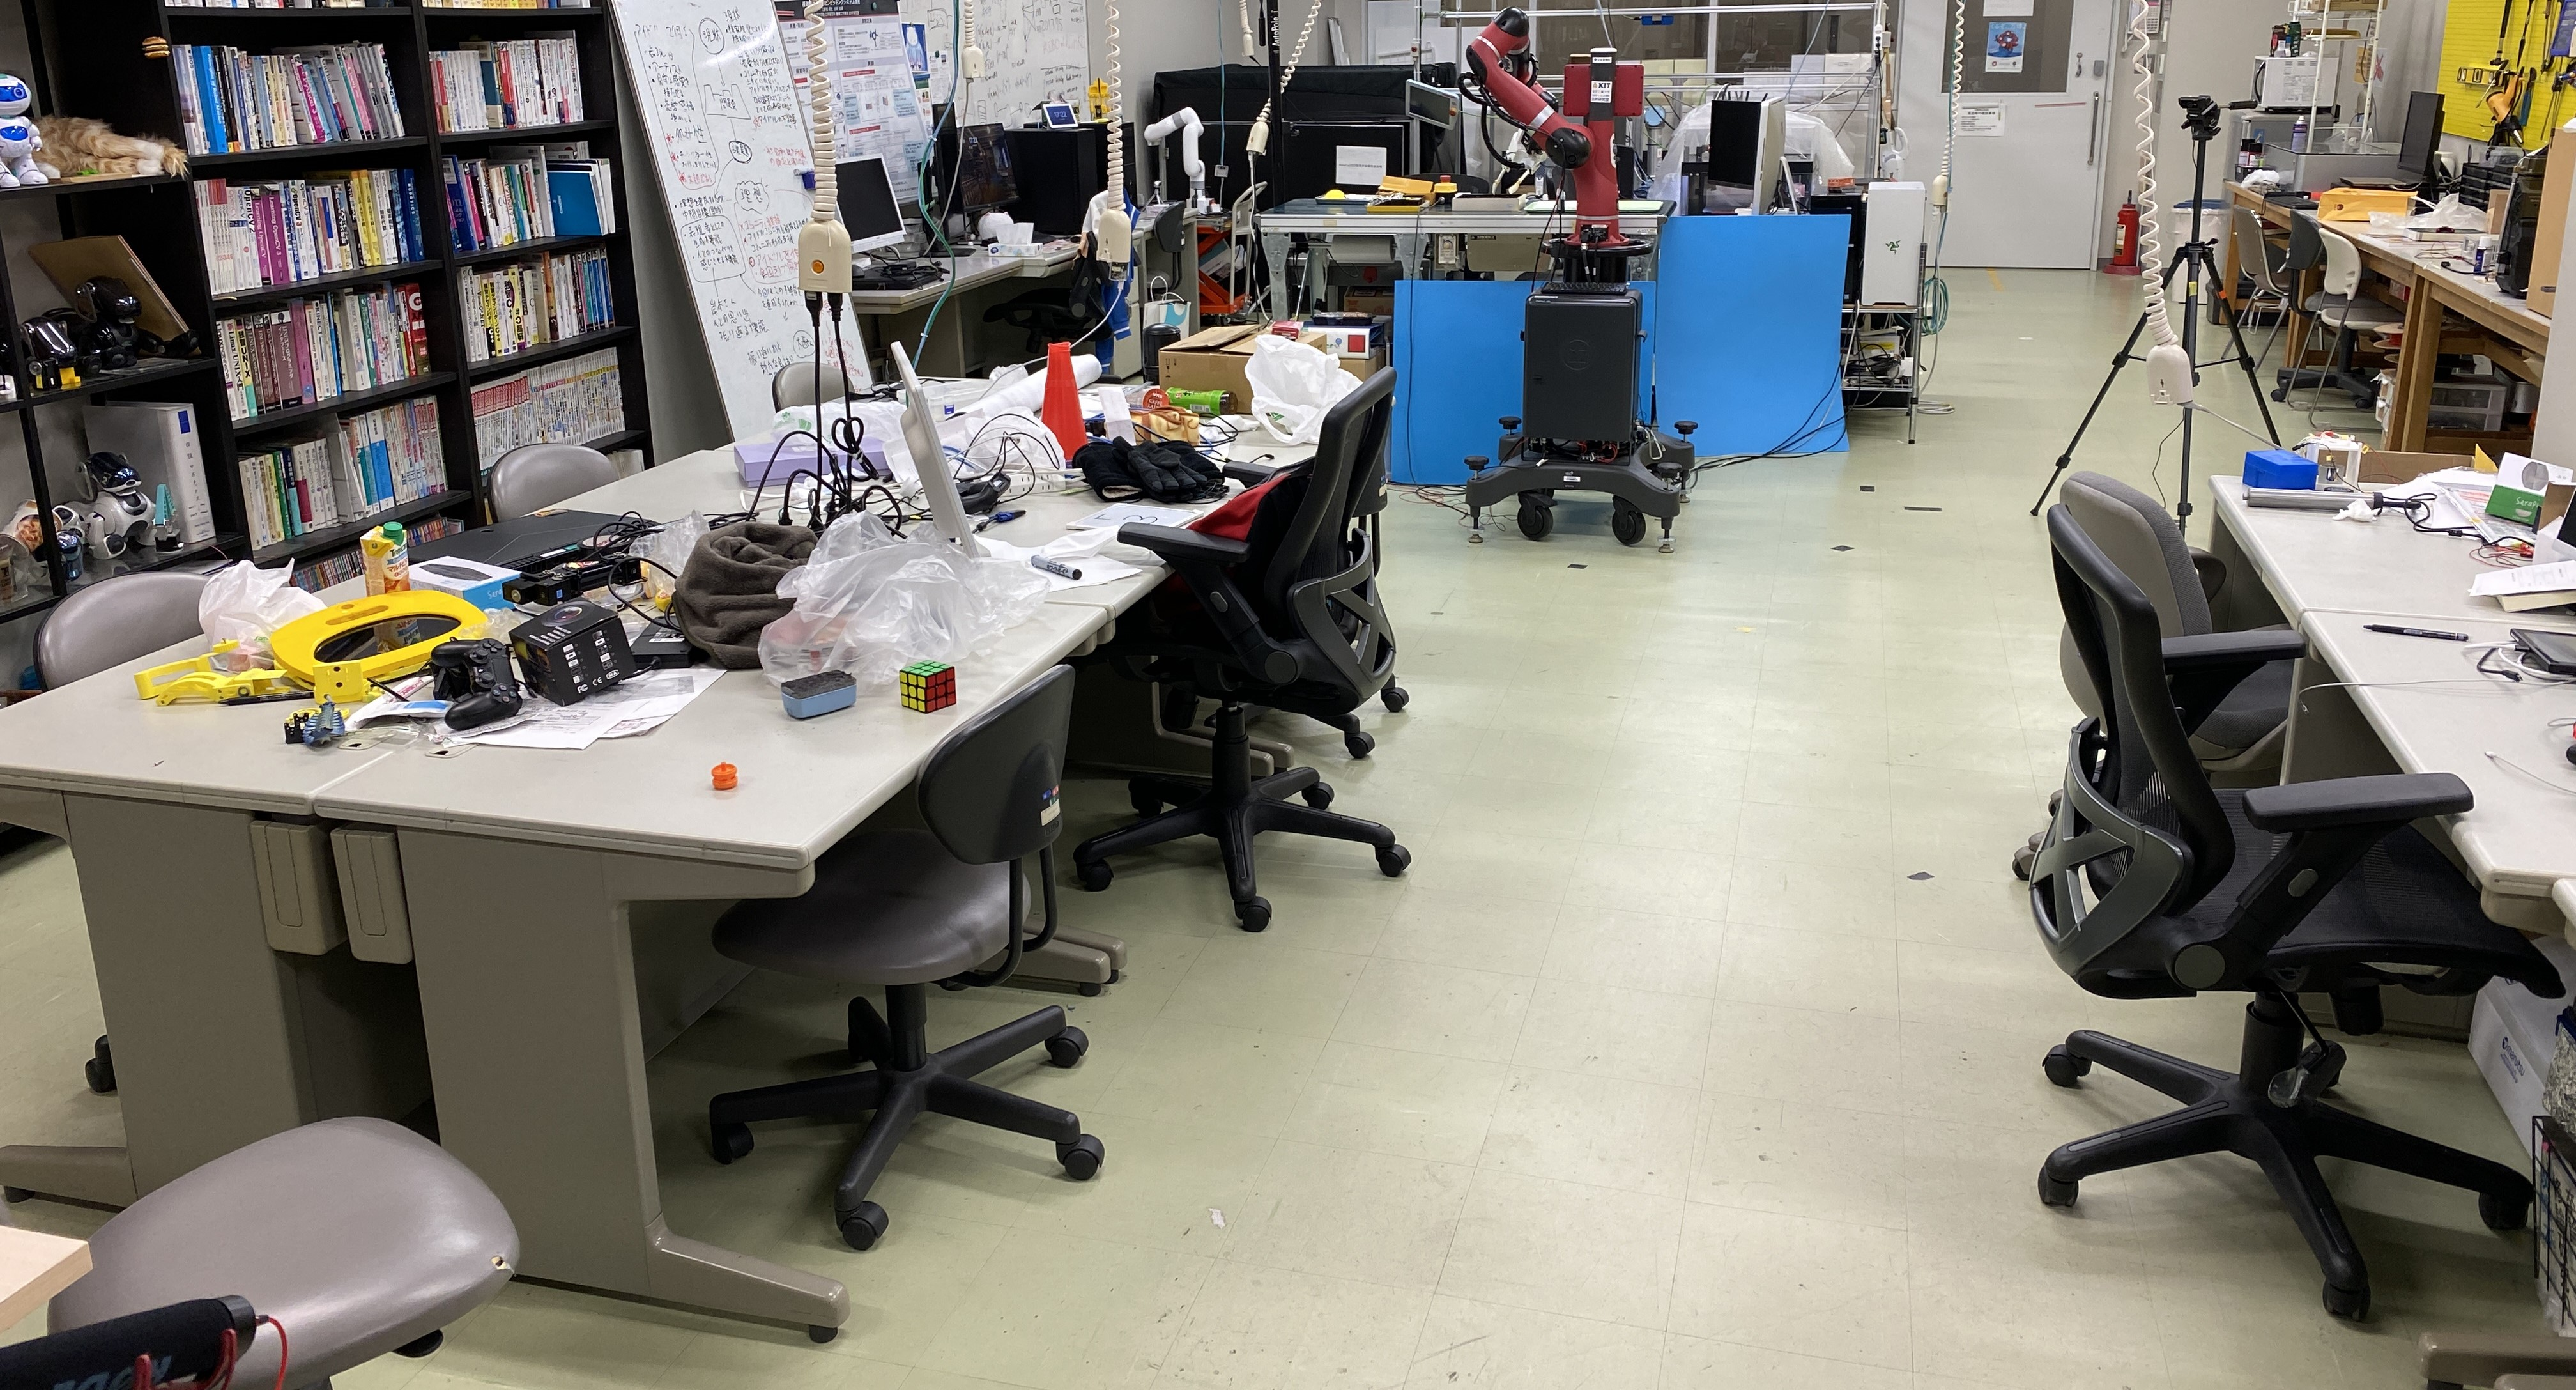
\includegraphics[width=150mm,clip]{figure/experimental_env1.JPG}
  \caption{Image of tracking experiment environment (FMT Laboratory Room 206)}
  \label{Image of tracking experiment environment (FMT Laboratory Room 206)}
  \end{center}
\end{figure*}

\begin{figure*}[h]
  \begin{center}
  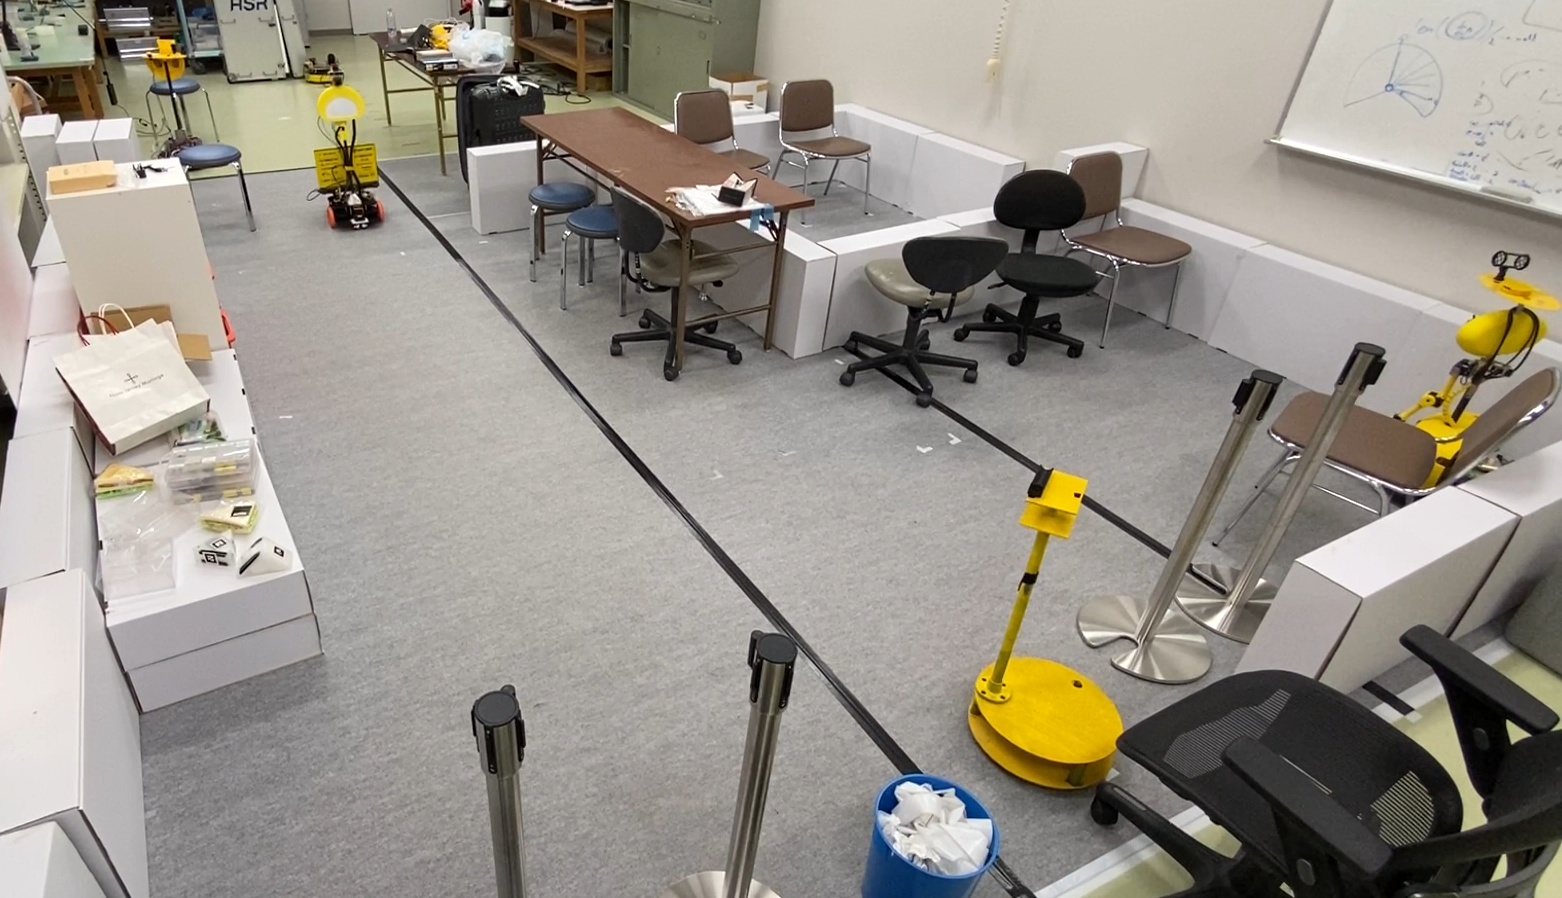
\includegraphics[width=150mm,clip]{figure/experimental_env2.png}
  \caption{Image of tracking experiment environment (FMT Laboratory Room 326)}
  \label{Image of tracking experiment environment (FMT Laboratory Room 326)}
  \end{center}
\end{figure*}

\begin{figure*}[h]
  \begin{center}
  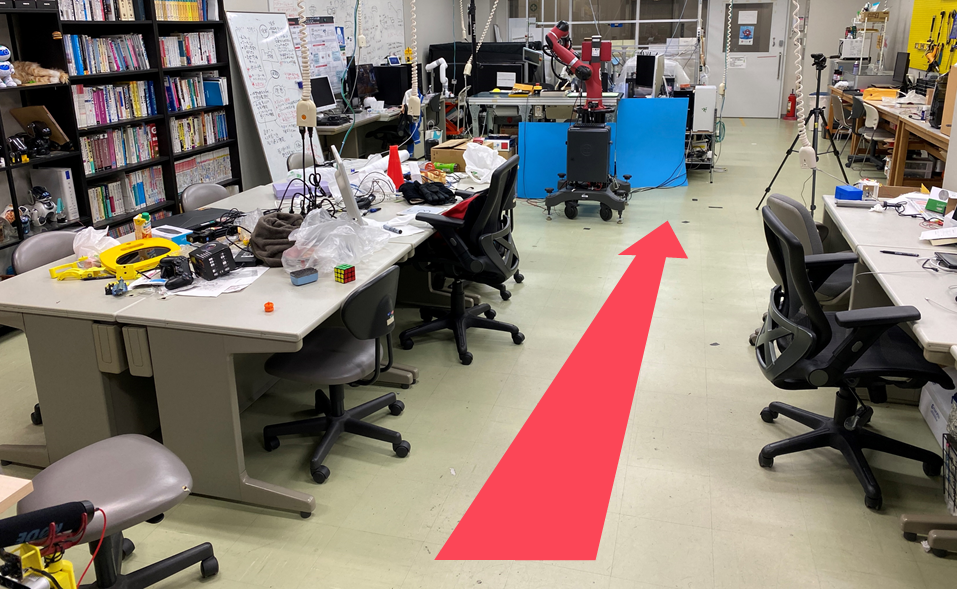
\includegraphics[width=100mm,clip]{figure/Straight.PNG}
  \caption{Straight road}
  \label{Straight road}
  \end{center}
\end{figure*}

\begin{figure*}[h]
  \begin{center}
  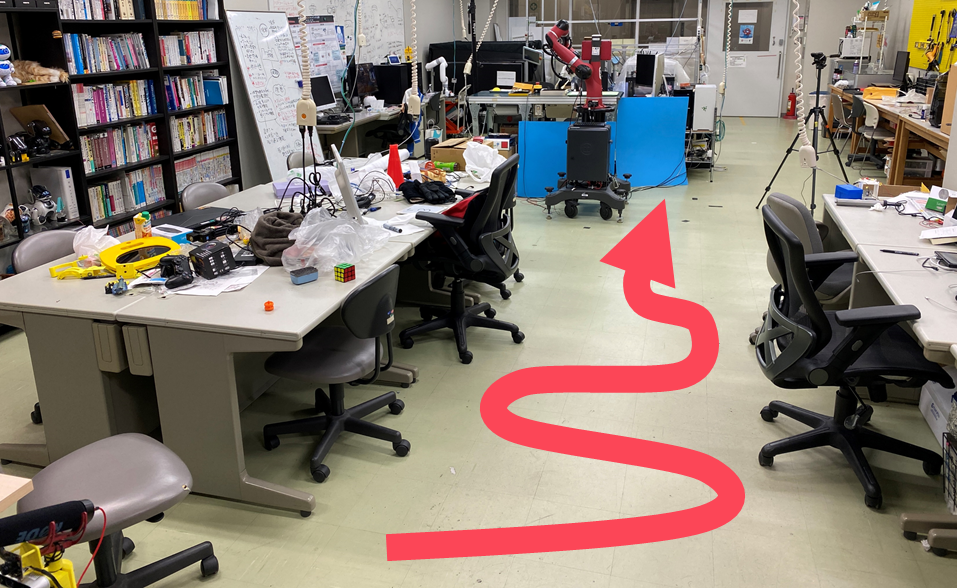
\includegraphics[width=100mm,clip]{figure/Curve.PNG}
  \caption{Curved road}
  \label{Curved road}
  \end{center}
\end{figure*}

\begin{figure*}[h]
  \begin{center}
  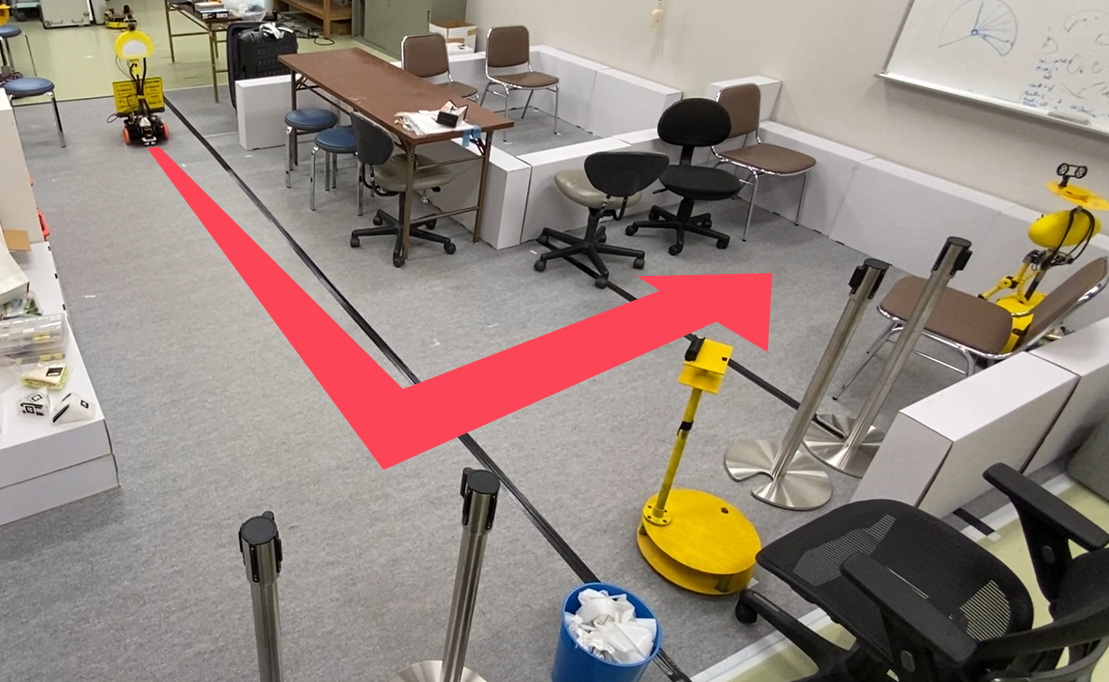
\includegraphics[width=100mm,clip]{figure/Right-angle.PNG}
  \caption{Right angle road}
  \label{Right angle road}
  \end{center}
\end{figure*}

\clearpage

\subsection{最大追従速度実験}
要求仕様(3)を検証するため、
Fig. \ref{Maximum tracking speed experiment environment image (FMT Laboratory Room 326)}
のような10[m]の直線経路を用意し最大追従速度を計測する。実験する速度は0.1[m/s]から開始し、
0.1ずつ速度を上昇させ、Happy Eduが追従できなくなった場合の1つ前の速度を最大追従速度とする。
追従の成否は、Happy Eduが追従対象者を10[m]以上追従したことを追従成功とする。
また、Happy Eduの追従速度は追従対象者の歩行速度に依存しており、
追従対象者の歩行速度を指定した速度にする必要がある。
そのため、Fig. \ref{Image of maximum tracking speed experiment}のような構成で実験
する。0.1[m/s]の場合であれば、Fig. \ref{Image of maximum tracking speed experiment}
の「Speed keeper」を0.1[m/s]で直進させ、「Speed keeper」に追従対象者が追従する。さらに、
追従対象者にHappy Eduが追従することで、指定した速度での実験をする。これを、0.1[m/s]から
開始し、Happy Eduが追従できなくなるまで試行を繰り返す。

\begin{figure*}[h]
  \begin{center}
  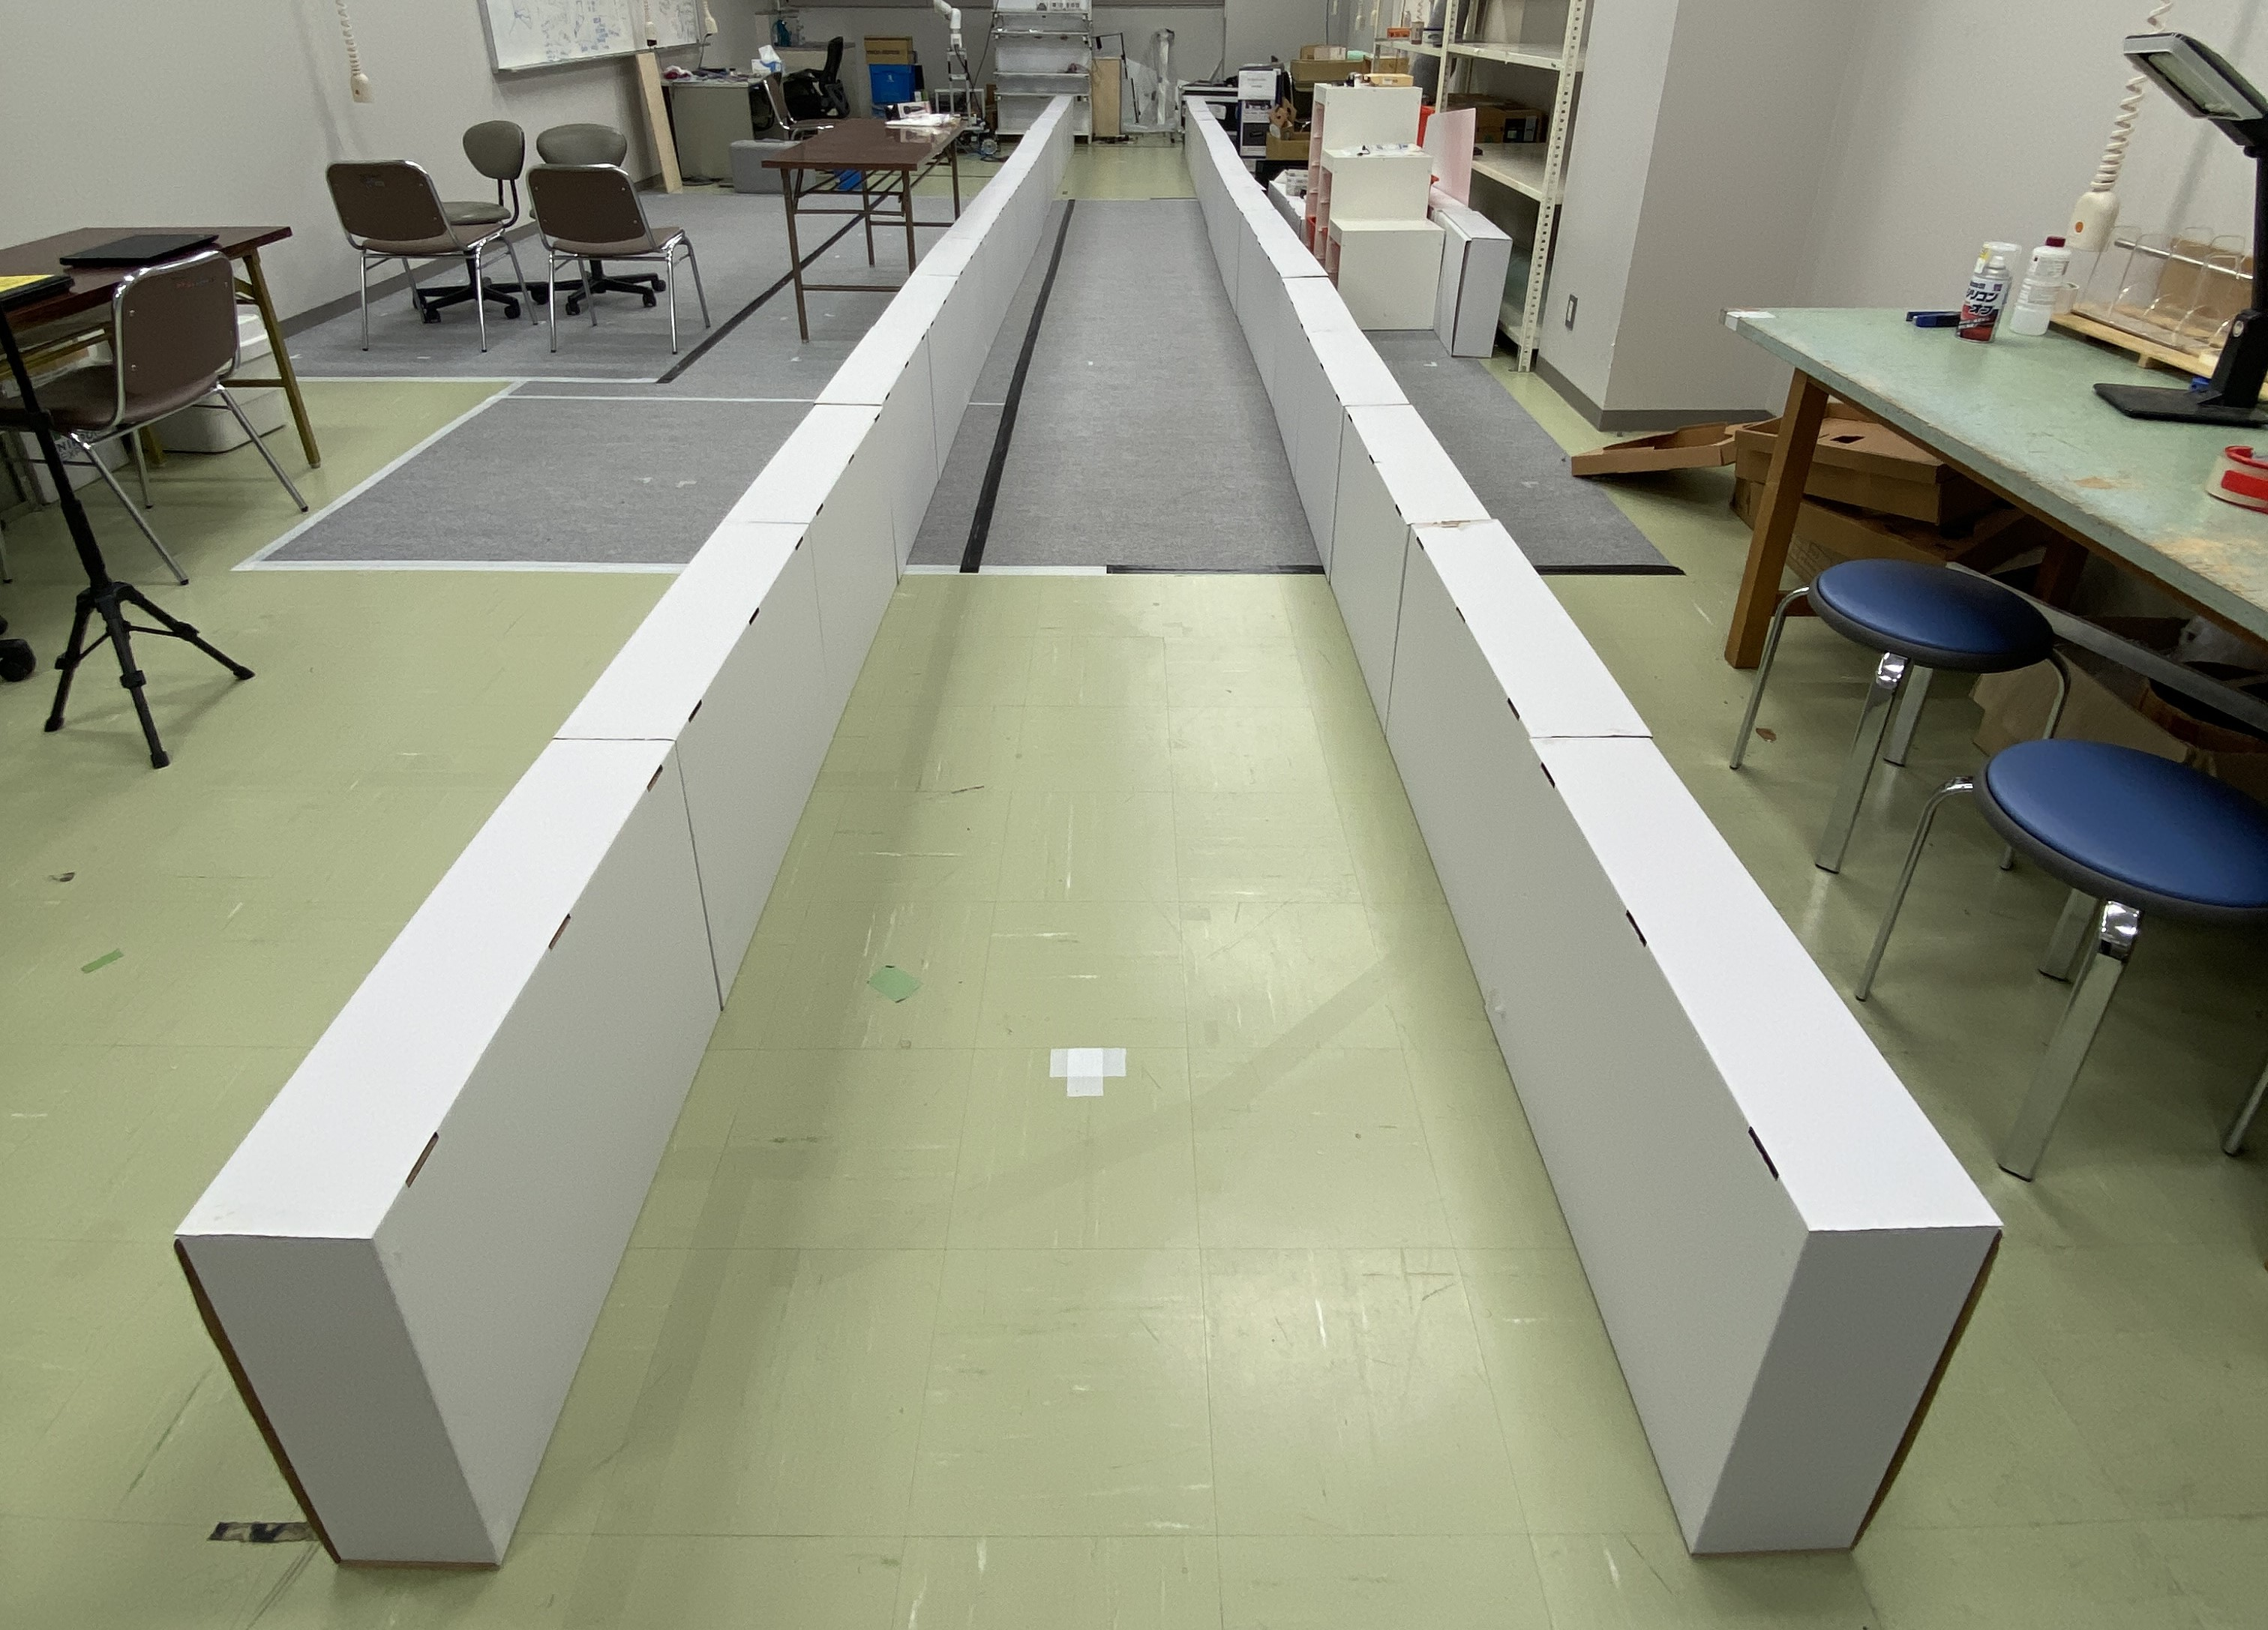
\includegraphics[width=80mm,clip]{figure/experimental_env3.JPG}
  \caption{Maximum tracking speed experiment environment image (FMT Laboratory Room 326)}
  \label{Maximum tracking speed experiment environment image (FMT Laboratory Room 326)}
  \end{center}
\end{figure*}

\begin{figure*}[h]
  \begin{center}
  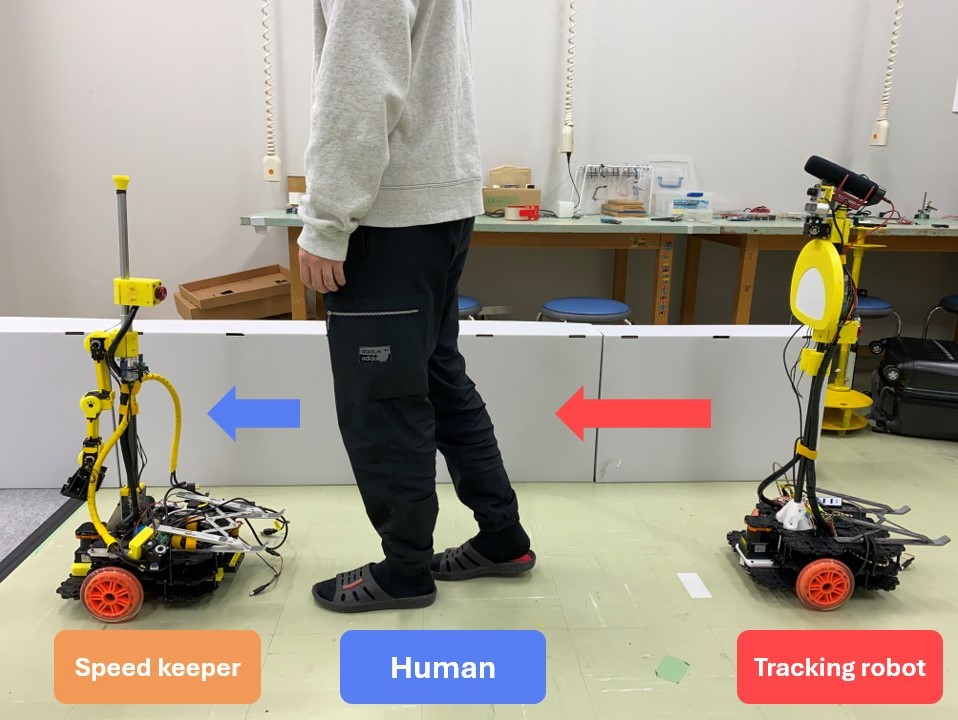
\includegraphics[width=90mm,clip]{figure/max_experiment_image.JPG}
  \caption{Image of maximum tracking speed experiment}
  \label{Image of maximum tracking speed experiment}
  \end{center}
\end{figure*}

\clearpage

\section{実験結果}
\subsection{追従実験}
追従実験の結果をTable \ref{Success rate of traking in each road}に示す。
追従実験では、直線経路、曲線経路、直角経路において、それぞれ10回ずつ試行し、計30回
の追従実験を試行したが、すべての試行において追従が成功した。\\ \indent
追従実験中の実世界での様子と同時刻におけるHappy Eduの内部処理の様子をそれぞれ、
Fig. \ref{Tracking experiment (Real view)}、
Fig. \ref{Tracking experiment (Internal view)}に示す。
Fig. \ref{Tracking experiment (Internal view)}から、追従対象者以外の物体を
誤検出していることがわかる。しかし、誤検出はしているが、提案手法の「追従目標の特定」
により正確に追従対象者を検出していることがわかる。
また、Fig. \ref{Tracking experiment (Real view)}より、
誤検出された物体は椅子の円柱部分であり、追従対象者の脚部と形状が類似している部分であった。

\begin{table}[h]
  \begin{center}
    \caption{{Success rate of traking in each road}\label{Success rate of traking in each road}}
    \scalebox{1.2}[1.0]{
      \begin{tabular}{c|r} \hline
        Road & Success rate [\%] \\ \hline
        Straight road & 100 \\
        Curved road & 100 \\
        Right angle road & 100 \\ \hline
      \end{tabular}
    }
  \end{center}
\end{table}

\begin{figure*}[h]
  \begin{minipage}[b]{0.45\linewidth}
    \centering
    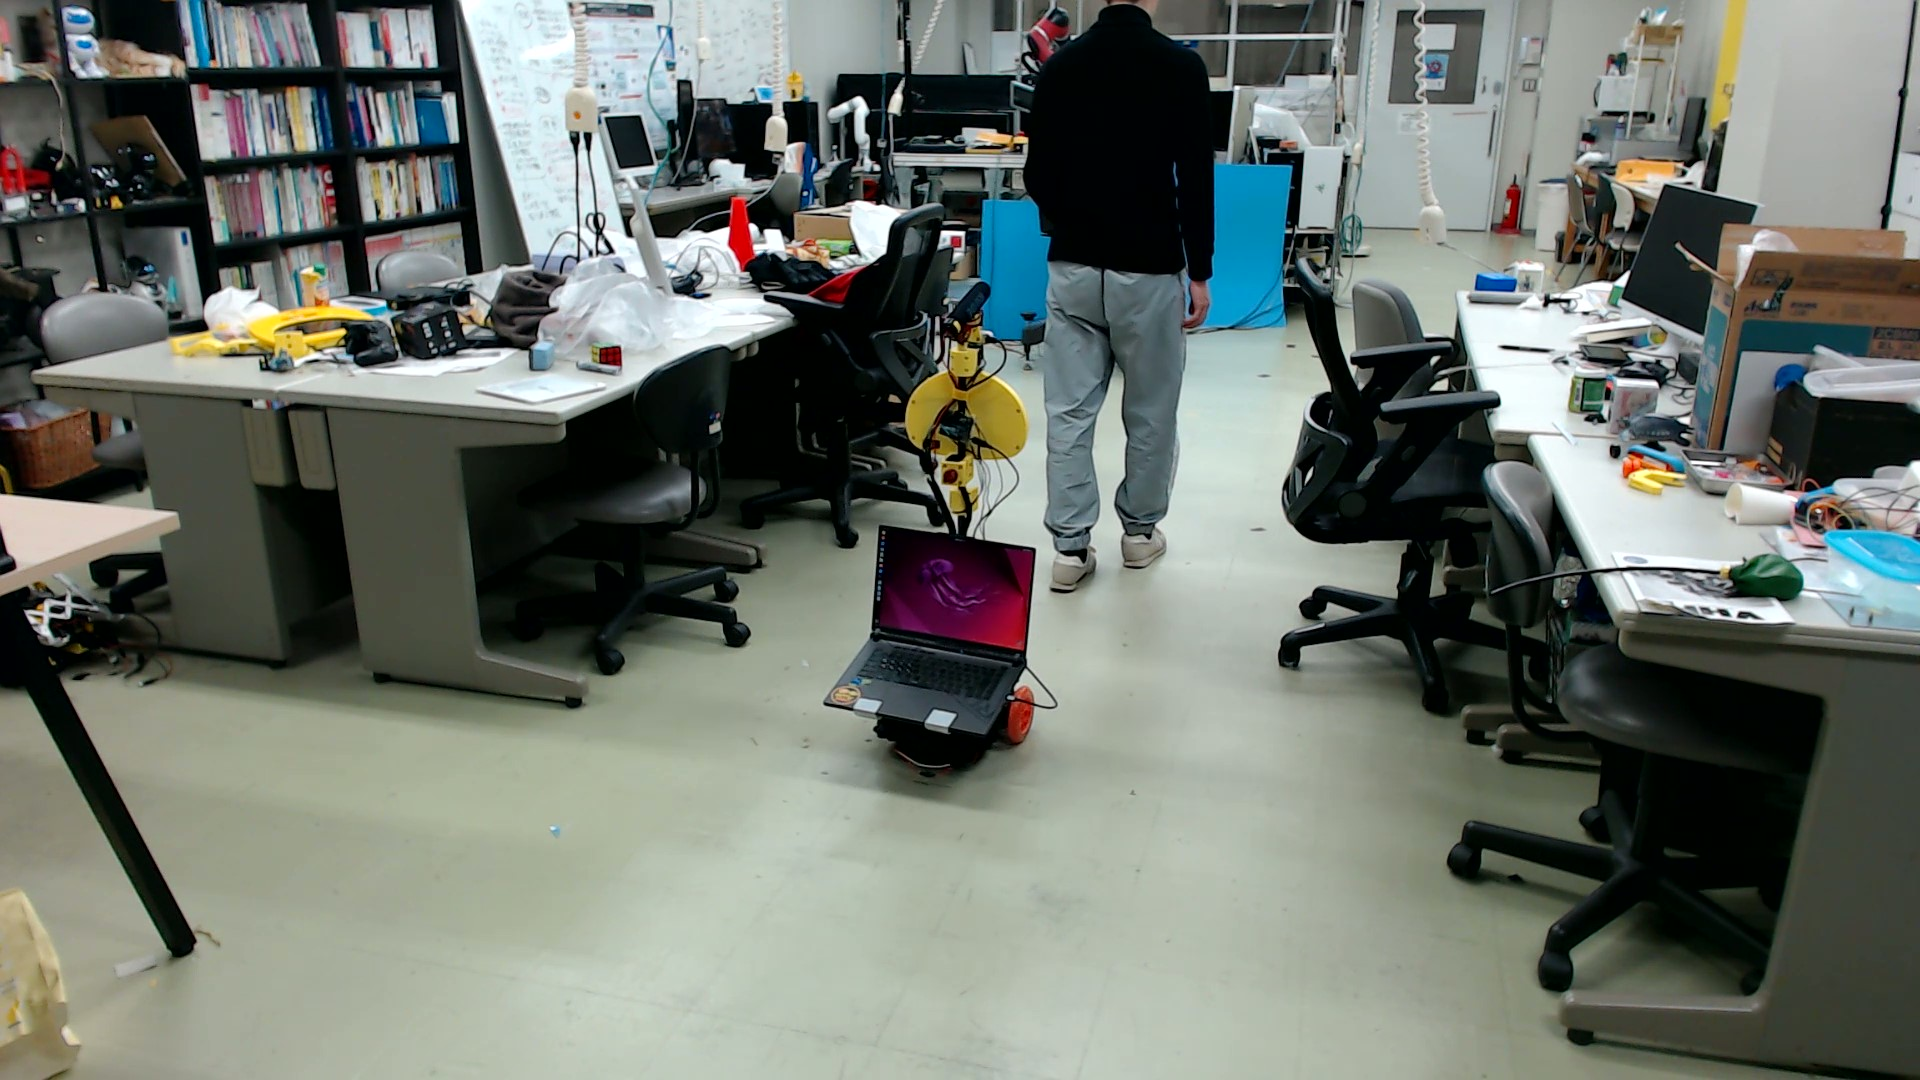
\includegraphics[keepaspectratio, scale=0.2]{figure/Tracking-experiment-Real-view.jpg}
    \caption{Tracking experiment (Real view)}
    \label{Tracking experiment (Real view)}
  \end{minipage}
  \begin{minipage}[b]{0.45\linewidth}
    \centering
    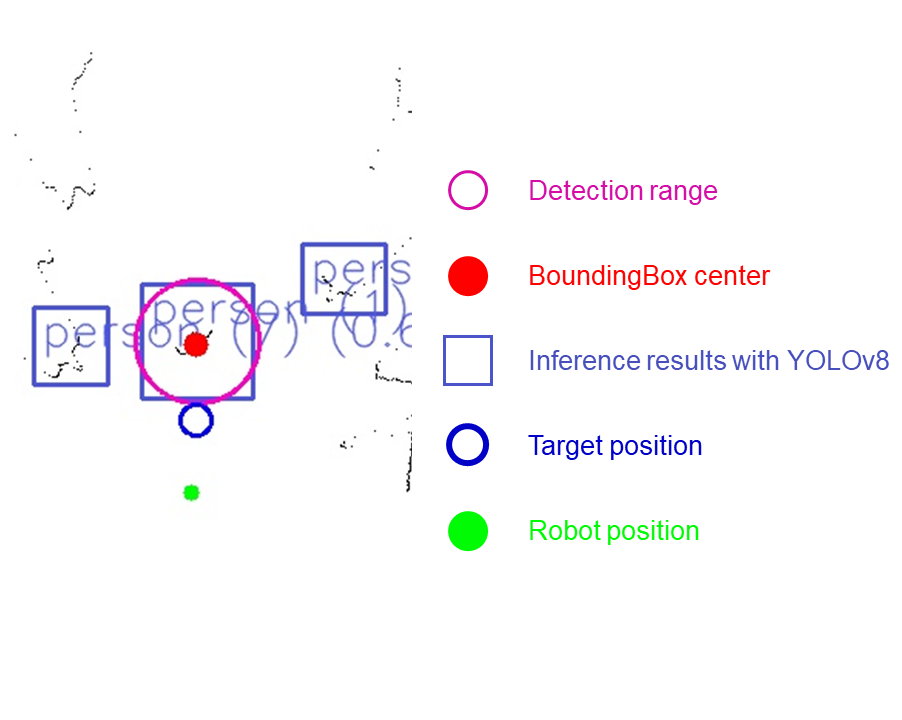
\includegraphics[keepaspectratio, scale=0.4]{figure/Tracking-experiment-Internal-view.png}
    \caption{Tracking experiment (Internal view)}
    \label{Tracking experiment (Internal view)}
  \end{minipage}
\end{figure*}

%\begin{figure*}[h]
%  \begin{center}
%  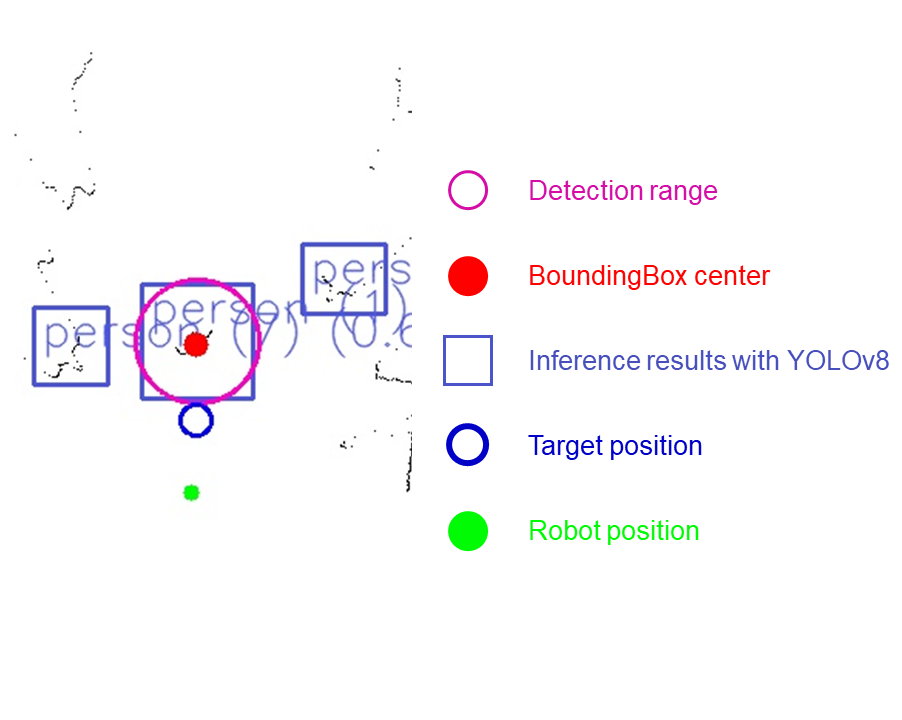
\includegraphics[width=170mm,clip]{figure/Tracking-experiment-Internal-view.png}
%  \caption{Tracking experiment (Internal view)}
%  \label{Tracking experiment (Internal view)}
%  \end{center}
%\end{figure*}

\subsection{最大追従速度実験}
最大追従速度実験の結果をTable \ref{Maximum tracking speed experimental result}と
Fig. \ref{Tracking speed graph}に示す。
Table \ref{Maximum tracking speed experimental result}より、0.1[m/s]~0.5[m/s]まで
は11[m]以上の追従が確認でき、0.6[m/s]では10[m]以上の追従が確認されなかった。
また、Fig. \ref{Tracking speed graph}より0.1[m/s]~0.5[m/s]では、Happy Eduから
追従対象者までの偏差が0.5[m]以下であるが、0.6[m/s]では追従対象者までの距離の偏差が
増加していき、6[m]付近で追従できなくなっていることが分かる。\\ \indent
以上より、本プロジェクトが提案する人追従システムの最大追従速度は0.5[m/s]であることがわかる。

\begin{table}[h]
  \begin{center}
    \caption{{Maximum tracking speed experimental result}\label{Maximum tracking speed experimental result}}
    \scalebox{1.0}[0.9]{
      \begin{tabular}{c|r} \hline
        Tracking speed [m/s] & Travel distance tracked [m] \\ \hline
        0.1 & 11.73 \\
        0.2 & 11.31 \\
        0.3 & 11.58 \\
        0.4 & 11.53 \\
        0.5 & 11.48 \\
        0.6 & 6.231 \\ \hline
      \end{tabular}
    }
  \end{center}
\end{table}

\begin{figure*}[h]
  \begin{center}
  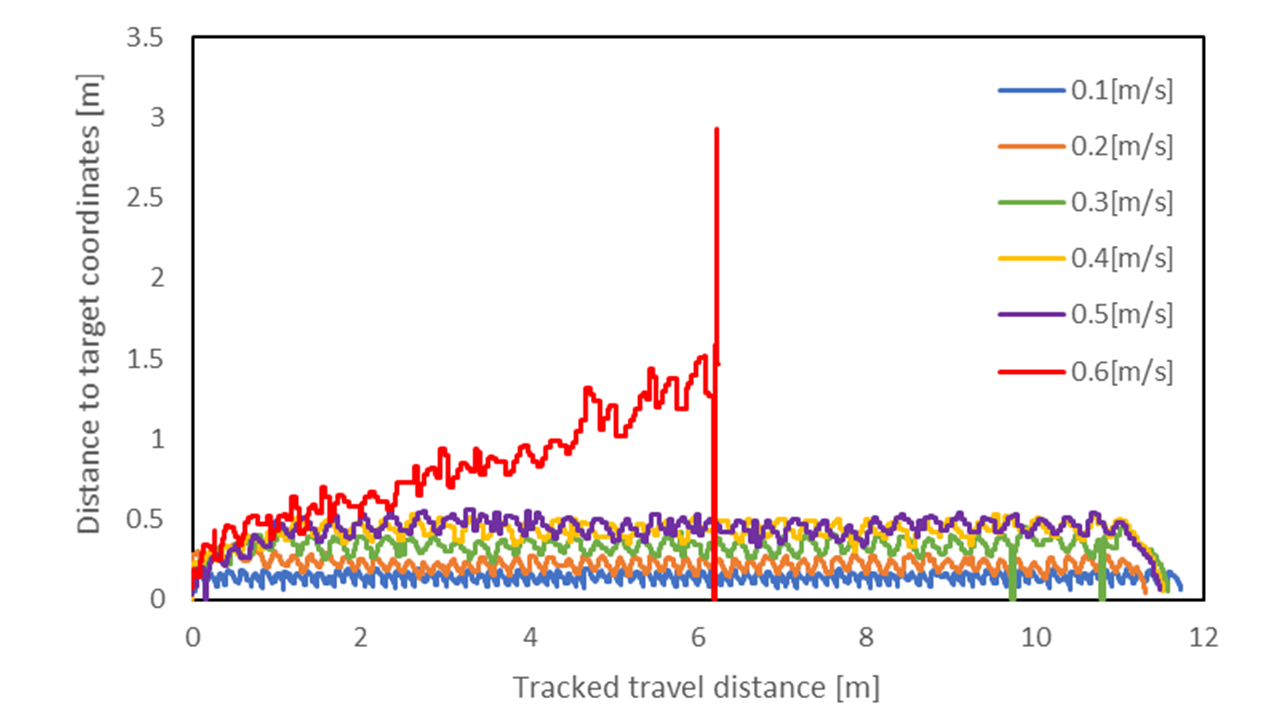
\includegraphics[width=150mm,clip]{figure/Maximum-tracking-speed-experimental-result.png}
  \caption{Tracking speed graph}
  \label{Tracking speed graph}
  \end{center}
\end{figure*}

\section{考察}
実験結果から、雑多な環境下での直線経路、曲線経路、直角経路において100[\%]の
人追従が確認されたため、要求仕様(2)を満たすことができた。
YOLOv8による両脚部の検出では、椅子などの物体を両脚部として誤検出していたが、
正確に追従対象者を追従できたのは、「追従目標の特定」により追従対象者を
正しく追跡できていることが考えられる。\\ \indent
最大追従速度実験では、最大追従速度が0.5[m/s]となり要求仕様(3)を満たすことができた。
最大追従速度が0.5[m/s]となった要因は、TurtleBot3 Big Wheelの最大直進速度が0.5[m/s]
であることに起因していると考えらる。このことから、本プロジェクトが提案する人追従システム
は、人の平均歩行速度以上の最大直進速度で移動できるロボット台車に実装することにより、
追従対象者がロボットに合わせて歩行速度を低下させる課題が解決できると考えられる。
